\documentclass[tikz,border=10pt]{standalone}
\usepackage[T1]{fontenc}
\usepackage{helvet}
\renewcommand{\familydefault}{\sfdefault}
\usepackage{amsmath,amssymb}
\usepackage{tikz}
\usetikzlibrary{calc,positioning,fit,arrows.meta,shapes.geometric}

% Canonical Academic Palette
\definecolor{OxfordNavy}{HTML}{1E293B}
\definecolor{SlateSteel}{HTML}{334155}
\definecolor{MutedTeal}{HTML}{0F766E}
\definecolor{TealL0}{HTML}{F0FDFA}
\definecolor{Burgundy}{HTML}{991B1B}
\definecolor{BurgundyL0}{HTML}{FEF2F2}
\definecolor{WarmOchre}{HTML}{92400E}
\definecolor{OchreL0}{HTML}{FFFBEB}
\definecolor{ForestSage}{HTML}{166534}
\definecolor{SageL0}{HTML}{F0FDF4}
\definecolor{CoolParchment}{HTML}{F8FAFC}
\definecolor{SlateRim}{HTML}{CBD5E1}
\definecolor{GridGray}{HTML}{E2E8F0}
\definecolor{DarkSlate}{HTML}{0F172A}
\definecolor{Amethyst}{HTML}{6B21A8}
\definecolor{AmethystL0}{HTML}{FAF5FF}

\begin{document}
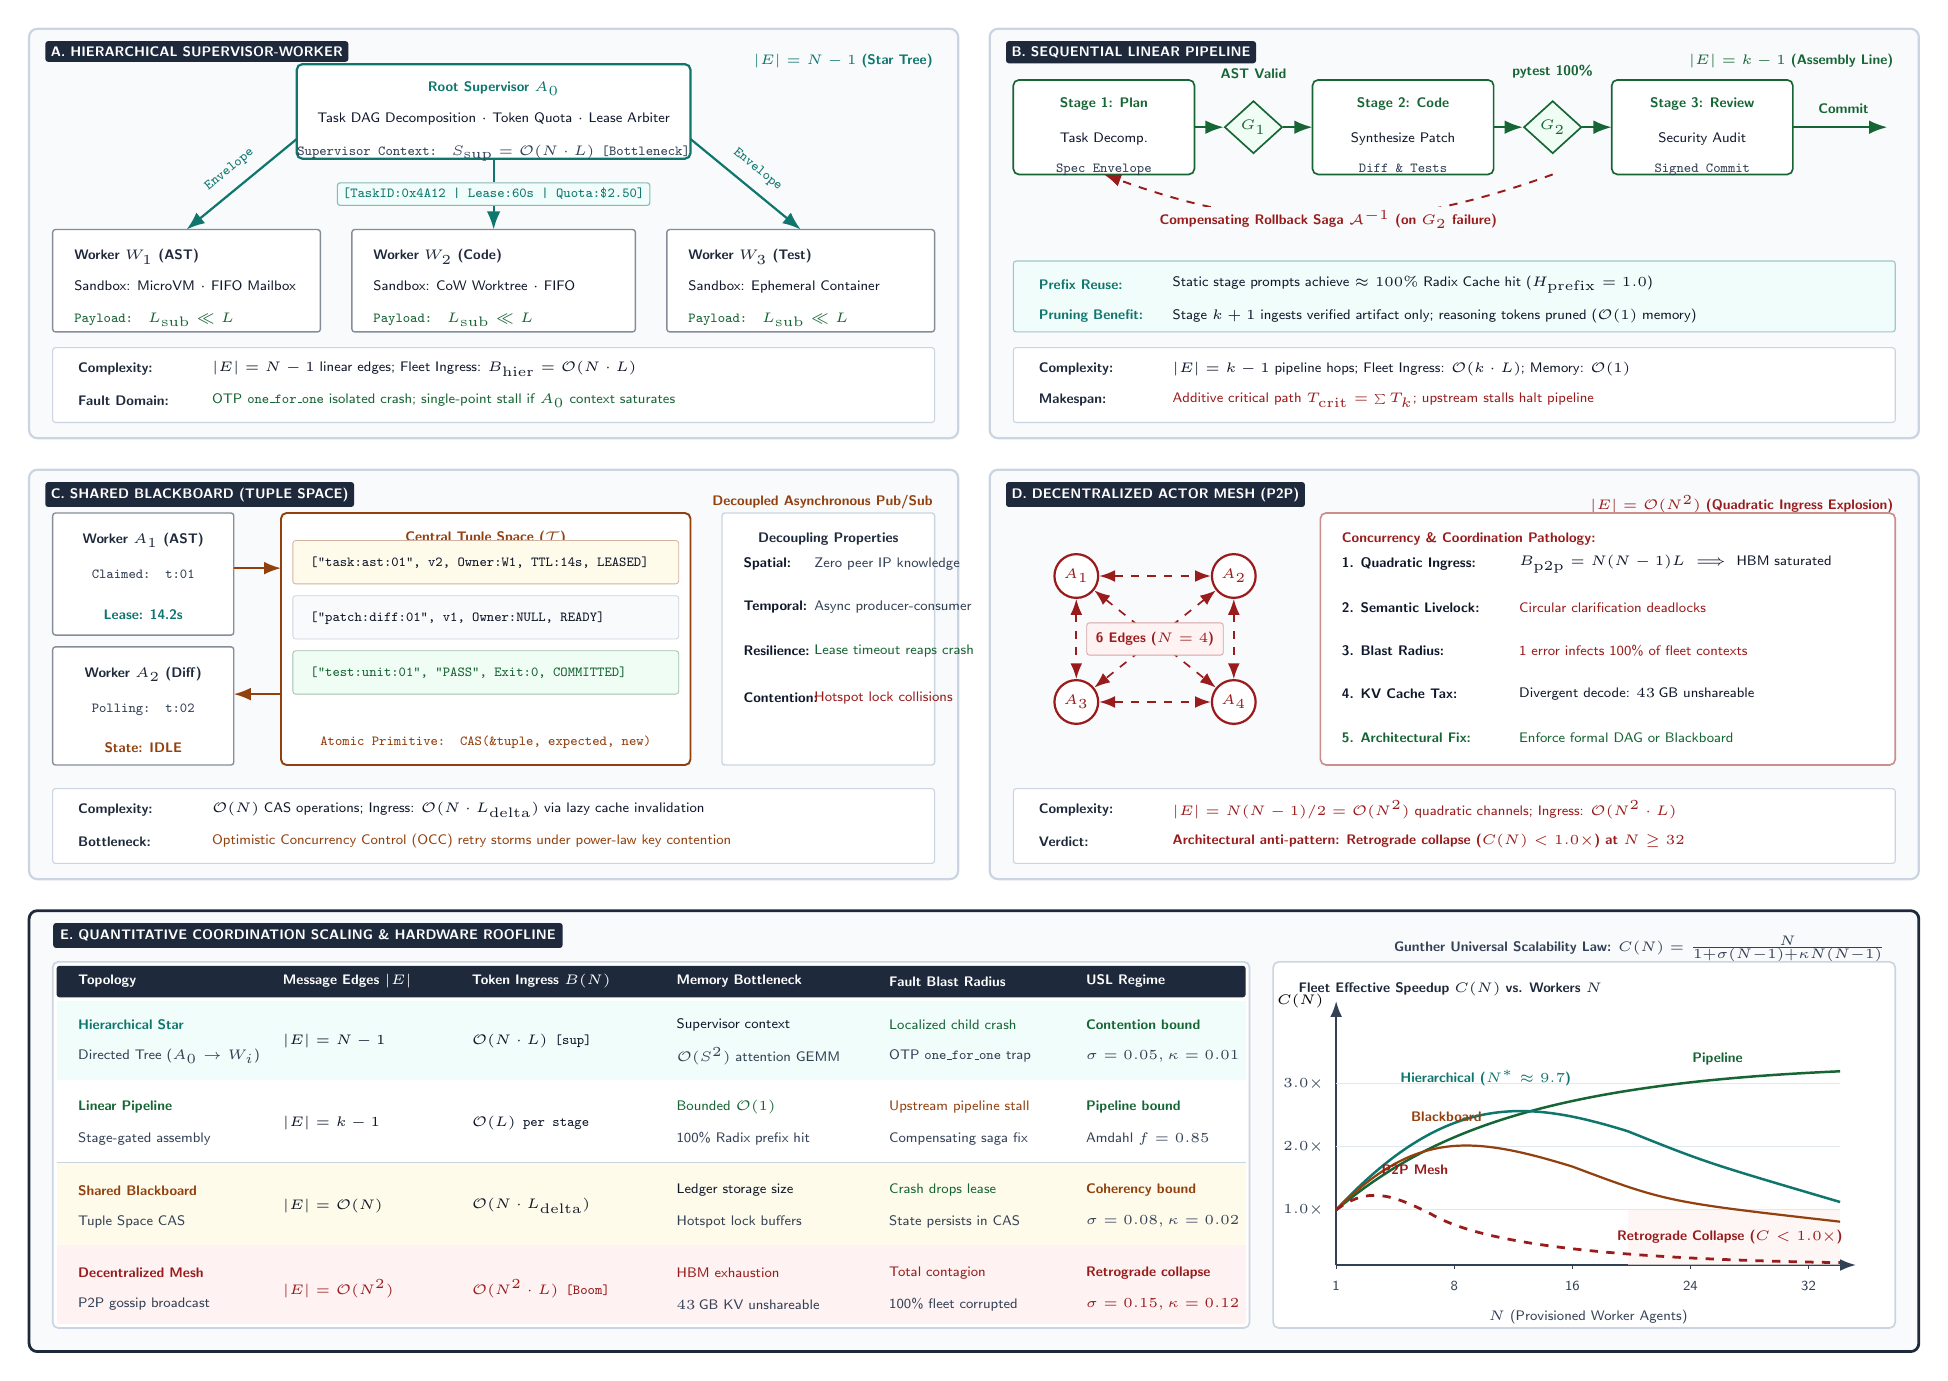
\begin{tikzpicture}[x=1cm, y=1cm, >=Latex]

% =============================================================================
% TOP SECTION: 2x2 ARCHITECTURAL TOPOLOGY GRID
% (x: 0 to 24.0, y: 6.0 to 16.8) - Height 10.8 cm
% =============================================================================

% -----------------------------------------------------------------------------
% PANEL (A): HIERARCHICAL SUPERVISOR-WORKER (Top-Left)
% x: 0 to 11.8, y: 11.6 to 16.8 (width 11.8, height 5.2 cm)
% -----------------------------------------------------------------------------
\begin{scope}[shift={(0, 11.6)}]
  \draw[fill=CoolParchment, draw=SlateRim, line width=0.8pt, rounded corners=3pt] (0, 0) rectangle (11.8, 5.2);
  
  % Badge
  \node[anchor=north west, fill=OxfordNavy, text=white, font=\fontsize{5.2}{6.2}\selectfont\bfseries, rounded corners=1pt, inner sep=2pt]
    at (0.2, 5.05) {A. HIERARCHICAL SUPERVISOR-WORKER};
  \node[anchor=north east, font=\fontsize{4.6}{5.4}\selectfont\bfseries, text=MutedTeal]
    at (11.6, 5.0) {$|E| = N - 1$ (Star Tree)};

  % Root Supervisor Node
  \draw[fill=white, draw=MutedTeal, line width=0.8pt, rounded corners=2pt] (3.4, 3.55) rectangle (8.4, 4.75);
  \node[anchor=north, font=\fontsize{4.8}{5.6}\selectfont\bfseries, text=MutedTeal] at (5.9, 4.65) {Root Supervisor $A_0$};
  \node[anchor=north, font=\fontsize{3.8}{4.5}\selectfont, text=DarkSlate] at (5.9, 4.25) {Task DAG Decomposition $\cdot$ Token Quota $\cdot$ Lease Arbiter};
  \node[anchor=north, font=\fontsize{3.6}{4.3}\selectfont\ttfamily, text=SlateSteel] at (5.9, 3.85) {Supervisor Context: $S_{\mathrm{sup}} = \mathcal{O}(N \cdot L)$ [Bottleneck]};

  % RPC Wire Packet Label (Compact 3.8cm box centered cleanly between A_0 and W_2)
  \node[fill=TealL0, draw=MutedTeal!50, line width=0.4pt, rounded corners=1pt, inner sep=2pt, font=\fontsize{3.4}{4.1}\selectfont\ttfamily, text=MutedTeal] (rpc) at (5.9, 3.10)
    {[TaskID:0x4A12 | Lease:60s | Quota:\$2.50]};

  % Three Sandboxed Workers
  % Worker 1
  \draw[fill=white, draw=SlateSteel!60, line width=0.5pt, rounded corners=1pt] (0.3, 1.35) rectangle (3.7, 2.65);
  \node[anchor=north west, font=\fontsize{4.4}{5.2}\selectfont\bfseries, text=OxfordNavy] at (0.45, 2.52) {Worker $W_1$ (AST)};
  \node[anchor=north west, font=\fontsize{3.6}{4.4}\selectfont, text=DarkSlate] at (0.45, 2.12) {Sandbox: MicroVM $\cdot$ FIFO Mailbox};
  \node[anchor=north west, font=\fontsize{3.5}{4.2}\selectfont\ttfamily, text=ForestSage] at (0.45, 1.72) {Payload: $L_{\mathrm{sub}} \ll L$};

  % Worker 2
  \draw[fill=white, draw=SlateSteel!60, line width=0.5pt, rounded corners=1pt] (4.1, 1.35) rectangle (7.7, 2.65);
  \node[anchor=north west, font=\fontsize{4.4}{5.2}\selectfont\bfseries, text=OxfordNavy] at (4.25, 2.52) {Worker $W_2$ (Code)};
  \node[anchor=north west, font=\fontsize{3.6}{4.4}\selectfont, text=DarkSlate] at (4.25, 2.12) {Sandbox: CoW Worktree $\cdot$ FIFO};
  \node[anchor=north west, font=\fontsize{3.5}{4.2}\selectfont\ttfamily, text=ForestSage] at (4.25, 1.72) {Payload: $L_{\mathrm{sub}} \ll L$};

  % Worker 3
  \draw[fill=white, draw=SlateSteel!60, line width=0.5pt, rounded corners=1pt] (8.1, 1.35) rectangle (11.5, 2.65);
  \node[anchor=north west, font=\fontsize{4.4}{5.2}\selectfont\bfseries, text=OxfordNavy] at (8.25, 2.52) {Worker $W_3$ (Test)};
  \node[anchor=north west, font=\fontsize{3.6}{4.4}\selectfont, text=DarkSlate] at (8.25, 2.12) {Sandbox: Ephemeral Container};
  \node[anchor=north west, font=\fontsize{3.5}{4.2}\selectfont\ttfamily, text=ForestSage] at (8.25, 1.72) {Payload: $L_{\mathrm{sub}} \ll L$};

  % Clean Dispatch Arrows (Clearances avoid colliding with RPC box)
  \draw[->, line width=0.8pt, draw=MutedTeal] (3.4, 3.8) -- node[above=1pt, sloped, font=\fontsize{3.2}{3.8}\selectfont\ttfamily, text=MutedTeal] {Envelope} (2.0, 2.65);
  \draw[line width=0.8pt, draw=MutedTeal] (5.9, 3.55) -- (rpc.north);
  \draw[->, line width=0.8pt, draw=MutedTeal] (rpc.south) -- (5.9, 2.65);
  \draw[->, line width=0.8pt, draw=MutedTeal] (8.4, 3.8) -- node[above=1pt, sloped, font=\fontsize{3.2}{3.8}\selectfont\ttfamily, text=MutedTeal] {Envelope} (9.8, 2.65);

  % Footer Metrics Strip
  \draw[fill=white, draw=SlateRim, line width=0.4pt, rounded corners=1pt] (0.3, 0.2) rectangle (11.5, 1.15);
  \node[anchor=west, font=\fontsize{3.8}{4.5}\selectfont\bfseries, text=OxfordNavy] at (0.5, 0.88) {Complexity:};
  \node[anchor=west, font=\fontsize{3.6}{4.4}\selectfont, text=DarkSlate] at (2.2, 0.88) {$|E| = N - 1$ linear edges; Fleet Ingress: $B_{\mathrm{hier}} = \mathcal{O}(N \cdot L)$};
  \node[anchor=west, font=\fontsize{3.8}{4.5}\selectfont\bfseries, text=OxfordNavy] at (0.5, 0.48) {Fault Domain:};
  \node[anchor=west, font=\fontsize{3.6}{4.4}\selectfont, text=ForestSage] at (2.2, 0.48) {OTP \texttt{one\_for\_one} isolated crash; single-point stall if $A_0$ context saturates};
\end{scope}

% -----------------------------------------------------------------------------
% PANEL (B): SEQUENTIAL LINEAR PIPELINE (Top-Right)
% x: 12.2 to 24.0, y: 11.6 to 16.8 (width 11.8, height 5.2 cm)
% -----------------------------------------------------------------------------
\begin{scope}[shift={(12.2, 11.6)}]
  \draw[fill=CoolParchment, draw=SlateRim, line width=0.8pt, rounded corners=3pt] (0, 0) rectangle (11.8, 5.2);
  
  % Badge
  \node[anchor=north west, fill=OxfordNavy, text=white, font=\fontsize{5.2}{6.2}\selectfont\bfseries, rounded corners=1pt, inner sep=2pt]
    at (0.2, 5.05) {B. SEQUENTIAL LINEAR PIPELINE};
  \node[anchor=north east, font=\fontsize{4.6}{5.4}\selectfont\bfseries, text=ForestSage]
    at (11.6, 5.0) {$|E| = k - 1$ (Assembly Line)};

  % Pipelined Stages & Gates (y center = 3.95)
  % Stage 1: Plan
  \draw[fill=white, draw=ForestSage, line width=0.6pt, rounded corners=2pt] (0.3, 3.35) rectangle (2.6, 4.55);
  \node[anchor=north, font=\fontsize{4.4}{5.2}\selectfont\bfseries, text=ForestSage] at (1.45, 4.45) {Stage 1: Plan};
  \node[anchor=north, font=\fontsize{3.6}{4.3}\selectfont, text=DarkSlate] at (1.45, 4.0) {Task Decomp.};
  \node[anchor=north, font=\fontsize{3.4}{4.1}\selectfont\ttfamily, text=SlateSteel] at (1.45, 3.6) {Spec Envelope};

  % Gate 1: AST Invariant
  \node[draw=ForestSage, fill=SageL0, line width=0.6pt, shape=diamond, aspect=1.1, inner sep=1.5pt] (g1) at (3.35, 3.95)
    {\fontsize{3.8}{4.5}\selectfont\bfseries\textcolor{ForestSage}{$G_1$}};
  \node[anchor=south, font=\fontsize{3.2}{3.8}\selectfont\bfseries, text=ForestSage] at (3.35, 4.45) {AST Valid};

  % Stage 2: Code
  \draw[fill=white, draw=ForestSage, line width=0.6pt, rounded corners=2pt] (4.1, 3.35) rectangle (6.4, 4.55);
  \node[anchor=north, font=\fontsize{4.4}{5.2}\selectfont\bfseries, text=ForestSage] at (5.25, 4.45) {Stage 2: Code};
  \node[anchor=north, font=\fontsize{3.6}{4.3}\selectfont, text=DarkSlate] at (5.25, 4.0) {Synthesize Patch};
  \node[anchor=north, font=\fontsize{3.4}{4.1}\selectfont\ttfamily, text=SlateSteel] at (5.25, 3.6) {Diff \& Tests};

  % Gate 2: Test Suite
  \node[draw=ForestSage, fill=SageL0, line width=0.6pt, shape=diamond, aspect=1.1, inner sep=1.5pt] (g2) at (7.15, 3.95)
    {\fontsize{3.8}{4.5}\selectfont\bfseries\textcolor{ForestSage}{$G_2$}};
  \node[anchor=south, font=\fontsize{3.2}{3.8}\selectfont\bfseries, text=ForestSage] at (7.15, 4.45) {pytest 100\%};

  % Stage 3: Review
  \draw[fill=white, draw=ForestSage, line width=0.6pt, rounded corners=2pt] (7.9, 3.35) rectangle (10.2, 4.55);
  \node[anchor=north, font=\fontsize{4.4}{5.2}\selectfont\bfseries, text=ForestSage] at (9.05, 4.45) {Stage 3: Review};
  \node[anchor=north, font=\fontsize{3.6}{4.3}\selectfont, text=DarkSlate] at (9.05, 4.0) {Security Audit};
  \node[anchor=north, font=\fontsize{3.4}{4.1}\selectfont\ttfamily, text=SlateSteel] at (9.05, 3.6) {Signed Commit};

  % Flow Arrows
  \draw[->, line width=0.8pt, draw=ForestSage] (2.6, 3.95) -- (g1.west);
  \draw[->, line width=0.8pt, draw=ForestSage] (g1.east) -- (4.1, 3.95);
  \draw[->, line width=0.8pt, draw=ForestSage] (6.4, 3.95) -- (g2.west);
  \draw[->, line width=0.8pt, draw=ForestSage] (g2.east) -- (7.9, 3.95);
  \draw[->, line width=0.8pt, draw=ForestSage] (10.2, 3.95) -- (11.4, 3.95);
  \node[anchor=west, font=\fontsize{3.4}{4.1}\selectfont\bfseries, text=ForestSage] at (10.4, 4.18) {Commit};

  % Compensating Rollback Saga Path (High clearance: arch dips from 3.35 down to 2.7, label at 2.7)
  \draw[->, line width=0.7pt, draw=Burgundy, dashed] (7.15, 3.35) to[out=-160, in=-20]
    node[midway, fill=CoolParchment, inner sep=1pt, font=\fontsize{3.3}{4.0}\selectfont\bfseries, text=Burgundy]
    {Compensating Rollback Saga $\mathcal{A}^{-1}$ (on $G_2$ failure)} (1.45, 3.35);

  % Radix Cache Prefix Strip (y: 1.35 to 2.25)
  \draw[fill=TealL0, draw=MutedTeal!40, line width=0.4pt, rounded corners=1pt] (0.3, 1.35) rectangle (11.5, 2.25);
  \node[anchor=west, font=\fontsize{3.8}{4.5}\selectfont\bfseries, text=MutedTeal] at (0.5, 1.95) {Prefix Reuse:};
  \node[anchor=west, font=\fontsize{3.6}{4.3}\selectfont, text=DarkSlate] at (2.2, 1.95) {Static stage prompts achieve $\approx 100\%$ Radix Cache hit ($H_{\mathrm{prefix}} = 1.0$)};
  \node[anchor=west, font=\fontsize{3.8}{4.5}\selectfont\bfseries, text=MutedTeal] at (0.5, 1.55) {Pruning Benefit:};
  \node[anchor=west, font=\fontsize{3.6}{4.3}\selectfont, text=DarkSlate] at (2.2, 1.55) {Stage $k+1$ ingests verified artifact only; reasoning tokens pruned ($\mathcal{O}(1)$ memory)};

  % Footer Metrics Strip
  \draw[fill=white, draw=SlateRim, line width=0.4pt, rounded corners=1pt] (0.3, 0.2) rectangle (11.5, 1.15);
  \node[anchor=west, font=\fontsize{3.8}{4.5}\selectfont\bfseries, text=OxfordNavy] at (0.5, 0.88) {Complexity:};
  \node[anchor=west, font=\fontsize{3.6}{4.4}\selectfont, text=DarkSlate] at (2.2, 0.88) {$|E| = k - 1$ pipeline hops; Fleet Ingress: $\mathcal{O}(k \cdot L)$; Memory: $\mathcal{O}(1)$};
  \node[anchor=west, font=\fontsize{3.8}{4.5}\selectfont\bfseries, text=OxfordNavy] at (0.5, 0.48) {Makespan:};
  \node[anchor=west, font=\fontsize{3.6}{4.4}\selectfont, text=Burgundy] at (2.2, 0.48) {Additive critical path $T_{\mathrm{crit}} = \sum T_k$; upstream stalls halt pipeline};
\end{scope}

% -----------------------------------------------------------------------------
% PANEL (C): SHARED BLACKBOARD / TUPLE SPACE (Bottom-Left)
% x: 0 to 11.8, y: 6.0 to 11.2 (width 11.8, height 5.2 cm)
% -----------------------------------------------------------------------------
\begin{scope}[shift={(0, 6.0)}]
  \draw[fill=CoolParchment, draw=SlateRim, line width=0.8pt, rounded corners=3pt] (0, 0) rectangle (11.8, 5.2);
  
  % Badge
  \node[anchor=north west, fill=OxfordNavy, text=white, font=\fontsize{5.2}{6.2}\selectfont\bfseries, rounded corners=1pt, inner sep=2pt]
    at (0.2, 5.05) {C. SHARED BLACKBOARD (TUPLE SPACE)};
  \node[anchor=north east, font=\fontsize{4.6}{5.4}\selectfont\bfseries, text=WarmOchre]
    at (11.6, 5.0) {Decoupled Asynchronous Pub/Sub};

  % Left: Decoupled Workers (height 1.5 cm each)
  \draw[fill=white, draw=SlateSteel!60, line width=0.5pt, rounded corners=1pt] (0.3, 3.1) rectangle (2.6, 4.65);
  \node[anchor=north, font=\fontsize{4.2}{5.0}\selectfont\bfseries, text=OxfordNavy] at (1.45, 4.52) {Worker $A_1$ (AST)};
  \node[anchor=north, font=\fontsize{3.4}{4.1}\selectfont\ttfamily, text=SlateSteel] at (1.45, 4.05) {Claimed: t:01};
  \node[anchor=north, font=\fontsize{3.2}{3.8}\selectfont\bfseries, text=MutedTeal] at (1.45, 3.55) {Lease: 14.2s};

  \draw[fill=white, draw=SlateSteel!60, line width=0.5pt, rounded corners=1pt] (0.3, 1.45) rectangle (2.6, 2.95);
  \node[anchor=north, font=\fontsize{4.2}{5.0}\selectfont\bfseries, text=OxfordNavy] at (1.45, 2.82) {Worker $A_2$ (Diff)};
  \node[anchor=north, font=\fontsize{3.4}{4.1}\selectfont\ttfamily, text=SlateSteel] at (1.45, 2.35) {Polling: t:02};
  \node[anchor=north, font=\fontsize{3.2}{3.8}\selectfont\bfseries, text=WarmOchre] at (1.45, 1.85) {State: IDLE};

  % Center: Shared Tuple Space Strip Map (height 3.2 cm)
  \draw[fill=white, draw=WarmOchre, line width=0.7pt, rounded corners=2pt] (3.2, 1.45) rectangle (8.4, 4.65);
  \node[anchor=north, font=\fontsize{4.6}{5.4}\selectfont\bfseries, text=WarmOchre] at (5.8, 4.55) {Central Tuple Space ($\mathcal{T}$)};

  % Tuple Row 1
  \draw[fill=OchreL0, draw=WarmOchre!40, line width=0.3pt, rounded corners=1pt] (3.35, 3.75) rectangle (8.25, 4.30);
  \node[anchor=west, font=\fontsize{3.5}{4.2}\selectfont\ttfamily, text=DarkSlate] at (3.45, 4.02)
    {["task:ast:01", v2, Owner:W1, TTL:14s, LEASED]};

  % Tuple Row 2
  \draw[fill=CoolParchment, draw=SlateRim, line width=0.3pt, rounded corners=1pt] (3.35, 3.05) rectangle (8.25, 3.60);
  \node[anchor=west, font=\fontsize{3.5}{4.2}\selectfont\ttfamily, text=DarkSlate] at (3.45, 3.32)
    {["patch:diff:01", v1, Owner:NULL, READY]};

  % Tuple Row 3
  \draw[fill=SageL0, draw=ForestSage!40, line width=0.3pt, rounded corners=1pt] (3.35, 2.35) rectangle (8.25, 2.90);
  \node[anchor=west, font=\fontsize{3.5}{4.2}\selectfont\ttfamily, text=ForestSage] at (3.45, 2.62)
    {["test:unit:01", "PASS", Exit:0, COMMITTED]};

  \node[anchor=north, font=\fontsize{3.4}{4.1}\selectfont\ttfamily\bfseries, text=WarmOchre] at (5.8, 1.95)
    {Atomic Primitive: CAS(\&tuple, expected, new)};

  % Arrows between Workers & Tuple Space
  \draw[->, line width=0.7pt, draw=WarmOchre] (2.6, 3.95) -- (3.2, 3.95);
  \draw[<-, line width=0.7pt, draw=WarmOchre] (2.6, 2.35) -- (3.2, 2.35);

  % Right: Concurrency Traits Box (height 3.2 cm)
  \draw[fill=white, draw=SlateRim, line width=0.5pt, rounded corners=1pt] (8.8, 1.45) rectangle (11.5, 4.65);
  \node[anchor=north, font=\fontsize{4.2}{5.0}\selectfont\bfseries, text=OxfordNavy] at (10.15, 4.52) {Decoupling Properties};
  \node[anchor=west, font=\fontsize{3.5}{4.2}\selectfont\bfseries, text=DarkSlate] at (8.95, 4.00) {Spatial:};
  \node[anchor=west, font=\fontsize{3.3}{4.0}\selectfont, text=SlateSteel] at (9.85, 4.00) {Zero peer IP knowledge};
  \node[anchor=west, font=\fontsize{3.5}{4.2}\selectfont\bfseries, text=DarkSlate] at (8.95, 3.45) {Temporal:};
  \node[anchor=west, font=\fontsize{3.3}{4.0}\selectfont, text=SlateSteel] at (9.85, 3.45) {Async producer-consumer};
  \node[anchor=west, font=\fontsize{3.5}{4.2}\selectfont\bfseries, text=DarkSlate] at (8.95, 2.90) {Resilience:};
  \node[anchor=west, font=\fontsize{3.3}{4.0}\selectfont, text=ForestSage] at (9.85, 2.90) {Lease timeout reaps crash};
  \node[anchor=west, font=\fontsize{3.5}{4.2}\selectfont\bfseries, text=DarkSlate] at (8.95, 2.30) {Contention:};
  \node[anchor=west, font=\fontsize{3.3}{4.0}\selectfont, text=Burgundy] at (9.85, 2.30) {Hotspot lock collisions};

  % Footer Metrics Strip
  \draw[fill=white, draw=SlateRim, line width=0.4pt, rounded corners=1pt] (0.3, 0.2) rectangle (11.5, 1.15);
  \node[anchor=west, font=\fontsize{3.8}{4.5}\selectfont\bfseries, text=OxfordNavy] at (0.5, 0.88) {Complexity:};
  \node[anchor=west, font=\fontsize{3.6}{4.4}\selectfont, text=DarkSlate] at (2.2, 0.88) {$\mathcal{O}(N)$ CAS operations; Ingress: $\mathcal{O}(N \cdot L_{\mathrm{delta}})$ via lazy cache invalidation};
  \node[anchor=west, font=\fontsize{3.8}{4.5}\selectfont\bfseries, text=OxfordNavy] at (0.5, 0.48) {Bottleneck:};
  \node[anchor=west, font=\fontsize{3.6}{4.4}\selectfont, text=WarmOchre] at (2.2, 0.48) {Optimistic Concurrency Control (OCC) retry storms under power-law key contention};
\end{scope}

% -----------------------------------------------------------------------------
% PANEL (D): DECENTRALIZED ACTOR MESH (Bottom-Right)
% x: 12.2 to 24.0, y: 6.0 to 11.2 (width 11.8, height 5.2 cm)
% -----------------------------------------------------------------------------
\begin{scope}[shift={(12.2, 6.0)}]
  \draw[fill=CoolParchment, draw=SlateRim, line width=0.8pt, rounded corners=3pt] (0, 0) rectangle (11.8, 5.2);
  
  % Badge
  \node[anchor=north west, fill=OxfordNavy, text=white, font=\fontsize{5.2}{6.2}\selectfont\bfseries, rounded corners=1pt, inner sep=2pt]
    at (0.2, 5.05) {D. DECENTRALIZED ACTOR MESH (P2P)};
  \node[anchor=north east, font=\fontsize{4.6}{5.4}\selectfont\bfseries, text=Burgundy]
    at (11.6, 5.0) {$|E| = \mathcal{O}(N^2)$ (Quadratic Ingress Explosion)};

  % Left: 4 P2P Nodes in Ring with Cross Links
  \begin{scope}[shift={(2.1, 3.05)}]
    \node[circle, fill=white, draw=Burgundy, line width=0.8pt, inner sep=2pt] (p1) at (-1.0, 0.8)
      {\fontsize{4.2}{5.0}\selectfont\bfseries\textcolor{Burgundy}{$A_1$}};
    \node[circle, fill=white, draw=Burgundy, line width=0.8pt, inner sep=2pt] (p2) at (1.0, 0.8)
      {\fontsize{4.2}{5.0}\selectfont\bfseries\textcolor{Burgundy}{$A_2$}};
    \node[circle, fill=white, draw=Burgundy, line width=0.8pt, inner sep=2pt] (p3) at (-1.0, -0.8)
      {\fontsize{4.2}{5.0}\selectfont\bfseries\textcolor{Burgundy}{$A_3$}};
    \node[circle, fill=white, draw=Burgundy, line width=0.8pt, inner sep=2pt] (p4) at (1.0, -0.8)
      {\fontsize{4.2}{5.0}\selectfont\bfseries\textcolor{Burgundy}{$A_4$}};

    % Bilateral Mesh Links
    \draw[<->, draw=Burgundy, dashed, line width=0.6pt] (p1) -- (p2);
    \draw[<->, draw=Burgundy, dashed, line width=0.6pt] (p1) -- (p3);
    \draw[<->, draw=Burgundy, dashed, line width=0.6pt] (p1) -- (p4);
    \draw[<->, draw=Burgundy, dashed, line width=0.6pt] (p2) -- (p3);
    \draw[<->, draw=Burgundy, dashed, line width=0.6pt] (p2) -- (p4);
    \draw[<->, draw=Burgundy, dashed, line width=0.6pt] (p3) -- (p4);

    \node[anchor=center, fill=BurgundyL0, draw=Burgundy!40, line width=0.3pt, rounded corners=1pt, font=\fontsize{3.2}{3.8}\selectfont\bfseries, text=Burgundy]
      at (0, 0) {6 Edges ($N=4$)};
  \end{scope}

  % Right: Failure Mechanics Card (width 7.3 cm, height 3.2 cm)
  \draw[fill=white, draw=Burgundy!50, line width=0.6pt, rounded corners=2pt] (4.2, 1.45) rectangle (11.5, 4.65);
  \node[anchor=north west, font=\fontsize{4.2}{5.0}\selectfont\bfseries, text=Burgundy] at (4.35, 4.52) {Concurrency \& Coordination Pathology:};

  \node[anchor=west, font=\fontsize{3.5}{4.2}\selectfont\bfseries, text=DarkSlate] at (4.35, 4.00) {1. Quadratic Ingress:};
  \node[anchor=west, font=\fontsize{3.3}{4.0}\selectfont, text=DarkSlate] at (6.6, 4.00) {$B_{\mathrm{p2p}} = N(N-1)L \implies$ HBM saturated};

  \node[anchor=west, font=\fontsize{3.5}{4.2}\selectfont\bfseries, text=DarkSlate] at (4.35, 3.45) {2. Semantic Livelock:};
  \node[anchor=west, font=\fontsize{3.3}{4.0}\selectfont, text=Burgundy] at (6.6, 3.45) {Circular clarification deadlocks};

  \node[anchor=west, font=\fontsize{3.5}{4.2}\selectfont\bfseries, text=DarkSlate] at (4.35, 2.90) {3. Blast Radius:};
  \node[anchor=west, font=\fontsize{3.3}{4.0}\selectfont, text=Burgundy] at (6.6, 2.90) {1 error infects 100\% of fleet contexts};

  \node[anchor=west, font=\fontsize{3.5}{4.2}\selectfont\bfseries, text=DarkSlate] at (4.35, 2.35) {4. KV Cache Tax:};
  \node[anchor=west, font=\fontsize{3.3}{4.0}\selectfont, text=DarkSlate] at (6.6, 2.35) {Divergent decode: $43\,\text{GB}$ unshareable};

  \node[anchor=west, font=\fontsize{3.5}{4.2}\selectfont\bfseries, text=ForestSage] at (4.35, 1.80) {5. Architectural Fix:};
  \node[anchor=west, font=\fontsize{3.3}{4.0}\selectfont, text=ForestSage] at (6.6, 1.80) {Enforce formal DAG or Blackboard};

  % Footer Metrics Strip
  \draw[fill=white, draw=SlateRim, line width=0.4pt, rounded corners=1pt] (0.3, 0.2) rectangle (11.5, 1.15);
  \node[anchor=west, font=\fontsize{3.8}{4.5}\selectfont\bfseries, text=OxfordNavy] at (0.5, 0.88) {Complexity:};
  \node[anchor=west, font=\fontsize{3.6}{4.4}\selectfont, text=Burgundy] at (2.2, 0.88) {$|E| = N(N-1)/2 = \mathcal{O}(N^2)$ quadratic channels; Ingress: $\mathcal{O}(N^2 \cdot L)$};
  \node[anchor=west, font=\fontsize{3.8}{4.5}\selectfont\bfseries, text=OxfordNavy] at (0.5, 0.48) {Verdict:};
  \node[anchor=west, font=\fontsize{3.6}{4.4}\selectfont\bfseries, text=Burgundy] at (2.2, 0.48) {Architectural anti-pattern: Retrograde collapse ($C(N) < 1.0\times$) at $N \ge 32$};
\end{scope}

% =============================================================================
% BOTTOM SECTION: SYSTEMS COORDINATION MATRIX & USL ROOFLINE
% (x: 0 to 24.0, y: 0 to 5.6) - Height 5.6 cm
% =============================================================================
\begin{scope}[shift={(0, 0)}]
  \draw[fill=CoolParchment, draw=OxfordNavy, line width=1.0pt, rounded corners=3pt] (0, 0) rectangle (24.0, 5.6);

  % Badge
  \node[anchor=north west, fill=OxfordNavy, text=white, font=\fontsize{5.5}{6.5}\selectfont\bfseries, rounded corners=1pt, inner sep=2.5pt]
    at (0.3, 5.45) {E. QUANTITATIVE COORDINATION SCALING \& HARDWARE ROOFLINE};
  \node[anchor=north east, font=\fontsize{4.6}{5.4}\selectfont\bfseries, text=SlateSteel]
    at (23.7, 5.4) {Gunther Universal Scalability Law: $C(N) = \frac{N}{1 + \sigma(N-1) + \kappa N(N-1)}$};

  % Left Part: Systems Scaling Matrix (x: 0.3 to 15.5, width 15.2 cm, height 4.65 cm)
  \begin{scope}[shift={(0.3, 0.3)}]
    \draw[fill=white, draw=SlateRim, line width=0.6pt, rounded corners=2pt] (0, 0) rectangle (15.2, 4.65);

    % Table Header
    \draw[fill=OxfordNavy, draw=none, rounded corners=1pt] (0.05, 4.2) rectangle (15.15, 4.6);
    \node[anchor=west, font=\fontsize{3.6}{4.4}\selectfont\bfseries, text=white] at (0.2, 4.4) {Topology};
    \node[anchor=west, font=\fontsize{3.6}{4.4}\selectfont\bfseries, text=white] at (2.8, 4.4) {Message Edges $|E|$};
    \node[anchor=west, font=\fontsize{3.6}{4.4}\selectfont\bfseries, text=white] at (5.2, 4.4) {Token Ingress $B(N)$};
    \node[anchor=west, font=\fontsize{3.6}{4.4}\selectfont\bfseries, text=white] at (7.8, 4.4) {Memory Bottleneck};
    \node[anchor=west, font=\fontsize{3.6}{4.4}\selectfont\bfseries, text=white] at (10.5, 4.4) {Fault Blast Radius};
    \node[anchor=west, font=\fontsize{3.6}{4.4}\selectfont\bfseries, text=white] at (13.0, 4.4) {USL Regime};

    % Row 1: Hierarchical Star
    \draw[fill=TealL0, draw=none] (0.05, 3.15) rectangle (15.15, 4.15);
    \node[anchor=west, font=\fontsize{3.8}{4.5}\selectfont\bfseries, text=MutedTeal] at (0.2, 3.85) {Hierarchical Star};
    \node[anchor=west, font=\fontsize{3.3}{4.0}\selectfont, text=SlateSteel] at (0.2, 3.45) {Directed Tree ($A_0 \to W_i$)};
    \node[anchor=west, font=\fontsize{3.5}{4.2}\selectfont\ttfamily, text=DarkSlate] at (2.8, 3.65) {$|E| = N - 1$};
    \node[anchor=west, font=\fontsize{3.5}{4.2}\selectfont\ttfamily, text=DarkSlate] at (5.2, 3.65) {$\mathcal{O}(N \cdot L)$ [sup]};
    \node[anchor=west, font=\fontsize{3.3}{4.0}\selectfont, text=DarkSlate] at (7.8, 3.85) {Supervisor context};
    \node[anchor=west, font=\fontsize{3.1}{3.8}\selectfont, text=SlateSteel] at (7.8, 3.45) {$\mathcal{O}(S^2)$ attention GEMM};
    \node[anchor=west, font=\fontsize{3.3}{4.0}\selectfont, text=ForestSage] at (10.5, 3.85) {Localized child crash};
    \node[anchor=west, font=\fontsize{3.1}{3.8}\selectfont, text=SlateSteel] at (10.5, 3.45) {OTP \texttt{one\_for\_one} trap};
    \node[anchor=west, font=\fontsize{3.3}{4.0}\selectfont\bfseries, text=ForestSage] at (13.0, 3.85) {Contention bound};
    \node[anchor=west, font=\fontsize{3.1}{3.8}\selectfont, text=SlateSteel] at (13.0, 3.45) {$\sigma=0.05, \kappa=0.01$};

    % Divider
    \draw[draw=SlateRim, line width=0.3pt] (0.05, 3.15) -- (15.15, 3.15);

    % Row 2: Linear Pipeline
    \draw[fill=white, draw=none] (0.05, 2.1) rectangle (15.15, 3.15);
    \node[anchor=west, font=\fontsize{3.8}{4.5}\selectfont\bfseries, text=ForestSage] at (0.2, 2.8) {Linear Pipeline};
    \node[anchor=west, font=\fontsize{3.3}{4.0}\selectfont, text=SlateSteel] at (0.2, 2.4) {Stage-gated assembly};
    \node[anchor=west, font=\fontsize{3.5}{4.2}\selectfont\ttfamily, text=DarkSlate] at (2.8, 2.6) {$|E| = k - 1$};
    \node[anchor=west, font=\fontsize{3.5}{4.2}\selectfont\ttfamily, text=DarkSlate] at (5.2, 2.6) {$\mathcal{O}(L)$ per stage};
    \node[anchor=west, font=\fontsize{3.3}{4.0}\selectfont, text=ForestSage] at (7.8, 2.8) {Bounded $\mathcal{O}(1)$};
    \node[anchor=west, font=\fontsize{3.1}{3.8}\selectfont, text=SlateSteel] at (7.8, 2.4) {100\% Radix prefix hit};
    \node[anchor=west, font=\fontsize{3.3}{4.0}\selectfont, text=WarmOchre] at (10.5, 2.8) {Upstream pipeline stall};
    \node[anchor=west, font=\fontsize{3.1}{3.8}\selectfont, text=SlateSteel] at (10.5, 2.4) {Compensating saga fix};
    \node[anchor=west, font=\fontsize{3.3}{4.0}\selectfont\bfseries, text=ForestSage] at (13.0, 2.8) {Pipeline bound};
    \node[anchor=west, font=\fontsize{3.1}{3.8}\selectfont, text=SlateSteel] at (13.0, 2.4) {Amdahl $f=0.85$};

    % Divider
    \draw[draw=SlateRim, line width=0.3pt] (0.05, 2.1) -- (15.15, 2.1);

    % Row 3: Shared Blackboard
    \draw[fill=OchreL0, draw=none] (0.05, 1.05) rectangle (15.15, 2.1);
    \node[anchor=west, font=\fontsize{3.8}{4.5}\selectfont\bfseries, text=WarmOchre] at (0.2, 1.75) {Shared Blackboard};
    \node[anchor=west, font=\fontsize{3.3}{4.0}\selectfont, text=SlateSteel] at (0.2, 1.35) {Tuple Space CAS};
    \node[anchor=west, font=\fontsize{3.5}{4.2}\selectfont\ttfamily, text=DarkSlate] at (2.8, 1.55) {$|E| = \mathcal{O}(N)$};
    \node[anchor=west, font=\fontsize{3.5}{4.2}\selectfont\ttfamily, text=DarkSlate] at (5.2, 1.55) {$\mathcal{O}(N \cdot L_{\mathrm{delta}})$};
    \node[anchor=west, font=\fontsize{3.3}{4.0}\selectfont, text=DarkSlate] at (7.8, 1.75) {Ledger storage size};
    \node[anchor=west, font=\fontsize{3.1}{3.8}\selectfont, text=SlateSteel] at (7.8, 1.35) {Hotspot lock buffers};
    \node[anchor=west, font=\fontsize{3.3}{4.0}\selectfont, text=ForestSage] at (10.5, 1.75) {Crash drops lease};
    \node[anchor=west, font=\fontsize{3.1}{3.8}\selectfont, text=SlateSteel] at (10.5, 1.35) {State persists in CAS};
    \node[anchor=west, font=\fontsize{3.3}{4.0}\selectfont\bfseries, text=WarmOchre] at (13.0, 1.75) {Coherency bound};
    \node[anchor=west, font=\fontsize{3.1}{3.8}\selectfont, text=SlateSteel] at (13.0, 1.35) {$\sigma=0.08, \kappa=0.02$};

    % Divider
    \draw[draw=SlateRim, line width=0.3pt] (0.05, 1.05) -- (15.15, 1.05);

    % Row 4: Decentralized Mesh
    \draw[fill=BurgundyL0, draw=none] (0.05, 0.05) rectangle (15.15, 1.05);
    \node[anchor=west, font=\fontsize{3.8}{4.5}\selectfont\bfseries, text=Burgundy] at (0.2, 0.7) {Decentralized Mesh};
    \node[anchor=west, font=\fontsize{3.3}{4.0}\selectfont, text=SlateSteel] at (0.2, 0.3) {P2P gossip broadcast};
    \node[anchor=west, font=\fontsize{3.5}{4.2}\selectfont\ttfamily, text=Burgundy] at (2.8, 0.5) {$|E| = \mathcal{O}(N^2)$};
    \node[anchor=west, font=\fontsize{3.5}{4.2}\selectfont\ttfamily, text=Burgundy] at (5.2, 0.5) {$\mathcal{O}(N^2 \cdot L)$ [Boom]};
    \node[anchor=west, font=\fontsize{3.3}{4.0}\selectfont, text=Burgundy] at (7.8, 0.7) {HBM exhaustion};
    \node[anchor=west, font=\fontsize{3.1}{3.8}\selectfont, text=SlateSteel] at (7.8, 0.3) {$43\,\text{GB}$ KV unshareable};
    \node[anchor=west, font=\fontsize{3.3}{4.0}\selectfont, text=Burgundy] at (10.5, 0.7) {Total contagion};
    \node[anchor=west, font=\fontsize{3.1}{3.8}\selectfont, text=SlateSteel] at (10.5, 0.3) {100\% fleet corrupted};
    \node[anchor=west, font=\fontsize{3.3}{4.0}\selectfont\bfseries, text=Burgundy] at (13.0, 0.7) {Retrograde collapse};
    \node[anchor=west, font=\fontsize{3.1}{3.8}\selectfont, text=Burgundy] at (13.0, 0.3) {$\sigma=0.15, \kappa=0.12$};
  \end{scope}

  % Right Part: Gunther USL Scaling Curves (x: 15.8 to 23.7, width 7.9 cm, height 4.65 cm)
  \begin{scope}[shift={(15.8, 0.3)}]
    \draw[fill=white, draw=SlateRim, line width=0.6pt, rounded corners=2pt] (0, 0) rectangle (7.9, 4.65);
    \node[anchor=north west, font=\fontsize{4.2}{5.0}\selectfont\bfseries, text=OxfordNavy] at (0.2, 4.52)
      {Fleet Effective Speedup $C(N)$ vs. Workers $N$};

    % Graph Axes
    % Origin: (0.8, 0.8), X max: (7.2, 0.8) width 6.4 cm (N: 1 to 32)
    % Y max: (0.8, 4.1) height 3.3 cm (C: 0 to 4.0x)
    \draw[->, draw=SlateSteel, line width=0.6pt] (0.8, 0.8) -- (7.4, 0.8);
    \draw[->, draw=SlateSteel, line width=0.6pt] (0.8, 0.8) -- (0.8, 4.15) node[left=1pt, font=\fontsize{3.4}{4.1}\selectfont] {$C(N)$};

    % Centered X Axis Label below ticks
    \node[anchor=north, font=\fontsize{3.4}{4.1}\selectfont, text=SlateSteel] at (4.0, 0.35) {$N$ (Provisioned Worker Agents)};

    % Ticks on Y
    \draw[draw=GridGray, line width=0.3pt] (0.8, 1.5) -- (7.2, 1.5);
    \node[left=1pt, font=\fontsize{3.0}{3.6}\selectfont, text=SlateSteel] at (0.8, 1.5) {$1.0\times$};
    \draw[draw=GridGray, line width=0.3pt] (0.8, 2.3) -- (7.2, 2.3);
    \node[left=1pt, font=\fontsize{3.0}{3.6}\selectfont, text=SlateSteel] at (0.8, 2.3) {$2.0\times$};
    \draw[draw=GridGray, line width=0.3pt] (0.8, 3.1) -- (7.2, 3.1);
    \node[left=1pt, font=\fontsize{3.0}{3.6}\selectfont, text=SlateSteel] at (0.8, 3.1) {$3.0\times$};

    % Ticks on X: N=1 (0.8), N=8 (2.3), N=16 (3.8), N=24 (5.3), N=32 (6.8)
    \draw[draw=SlateSteel, line width=0.4pt] (0.8, 0.75) -- (0.8, 0.8);
    \node[below=1pt, font=\fontsize{3.0}{3.6}\selectfont, text=SlateSteel] at (0.8, 0.75) {1};
    \draw[draw=SlateSteel, line width=0.4pt] (2.3, 0.75) -- (2.3, 0.8);
    \node[below=1pt, font=\fontsize{3.0}{3.6}\selectfont, text=SlateSteel] at (2.3, 0.75) {8};
    \draw[draw=SlateSteel, line width=0.4pt] (3.8, 0.75) -- (3.8, 0.8);
    \node[below=1pt, font=\fontsize{3.0}{3.6}\selectfont, text=SlateSteel] at (3.8, 0.75) {16};
    \draw[draw=SlateSteel, line width=0.4pt] (5.3, 0.75) -- (5.3, 0.8);
    \node[below=1pt, font=\fontsize{3.0}{3.6}\selectfont, text=SlateSteel] at (5.3, 0.75) {24};
    \draw[draw=SlateSteel, line width=0.4pt] (6.8, 0.75) -- (6.8, 0.8);
    \node[below=1pt, font=\fontsize{3.0}{3.6}\selectfont, text=SlateSteel] at (6.8, 0.75) {32};

    % Retrograde Collapse Shading: where C(N) < 1.0x (y: 0.8 to 1.5, x: 4.5 to 7.2)
    \draw[fill=BurgundyL0, draw=none, opacity=0.7] (4.5, 0.8) rectangle (7.2, 1.5);
    \node[anchor=center, font=\fontsize{3.0}{3.6}\selectfont\bfseries, text=Burgundy] at (5.8, 1.15) {Retrograde Collapse ($C < 1.0\times$)};

    % Curve 1: Linear Pipeline (Amdahl f=0.85, plateaus at ~3.26x)
    \draw[draw=ForestSage, line width=0.9pt]
      (0.8, 1.5) .. controls (2.0, 2.5) and (3.5, 3.1) .. (7.2, 3.26);
    \node[anchor=west, font=\fontsize{3.2}{3.8}\selectfont\bfseries, text=ForestSage] at (5.2, 3.42) {Pipeline};

    % Curve 2: Hierarchical Star (USL sigma=0.05, kappa=0.01, peak at N* ~ 9.7, C* ~ 2.7x)
    \draw[draw=MutedTeal, line width=0.9pt]
      (0.8, 1.5) .. controls (2.2, 3.0) and (3.2, 2.9) .. (4.5, 2.5) .. controls (5.5, 2.1) .. (7.2, 1.6);
    \node[anchor=south, font=\fontsize{3.2}{3.8}\selectfont\bfseries, text=MutedTeal] at (2.7, 2.95) {Hierarchical ($N^* \approx 9.7$)};

    % Curve 3: Shared Blackboard (USL sigma=0.08, kappa=0.02, peak at N* ~ 6.7, C* ~ 2.2x)
    \draw[draw=WarmOchre, line width=0.8pt]
      (0.8, 1.5) .. controls (1.8, 2.5) and (2.5, 2.45) .. (3.8, 2.05) .. controls (5.0, 1.6) .. (7.2, 1.35);
    \node[anchor=south, font=\fontsize{3.0}{3.6}\selectfont\bfseries, text=WarmOchre] at (2.2, 2.5) {Blackboard};

    % Curve 4: Decentralized Mesh (USL sigma=0.15, kappa=0.12, peak at N* ~ 2.6, C* ~ 1.4x, drops < 1.0x at N=6)
    \draw[draw=Burgundy, line width=1.0pt, dashed]
      (0.8, 1.5) .. controls (1.2, 1.8) and (1.5, 1.7) .. (2.0, 1.45) .. controls (2.6, 1.1) and (4.0, 0.88) .. (7.2, 0.83);
    \node[anchor=south, font=\fontsize{3.2}{3.8}\selectfont\bfseries, text=Burgundy] at (1.8, 1.82) {P2P Mesh};
  \end{scope}
\end{scope}

\end{tikzpicture}
\end{document}
